\documentclass{article}



% Package for rerunfilecheck error
\usepackage{bookmark}


% Packages for figures and equations
\usepackage{graphicx}
\usepackage{amsmath}



% Packages for algorithms
\usepackage{algorithm}
\usepackage{algpseudocode}
\usepackage{subfigure}

% Package for references
\usepackage{cite}
\usepackage{hyperref}
\usepackage{sectsty}
\begin{document}

% Formatting for headings
\sectionfont{\bfseries\uppercase}
% Title and author
\title{\textbf{\uppercase{JOINT DOA ESTIMATION AND SOURCE SIGNAL ESTIMATION WITH KALMAN FILTERING AND REGULARIZED QRD-RLS ALGORITHM - Paper Analysis}}}
\author{Harutjun Magakian}
\date{\today}
\maketitle


\section{Abstract}



This report covers my analysis and implementation of the algorithms provided in the paper with the title "Joint DOA Estimation and Source Signal Estimation with Kalman Filtering and Regularized QRD-RLS Algorithm"
by Jian-Feng Gu, S. C. Chan, Wei-Ping Zhu and M.N.S Swamy \cite{DOA_Kalman_RQRDRLS}.
The paper was published in the IEEE Transactions on Circuits and Systems in January 2013.
The paper presents a novel algorithm for joint direction-of-arrival (DOA) estimation and tracking and source signal estimation for multiple sources
The algorithm combines the Kalman filter and the regularized QR-decomposition recursive least squares (QRD-RLS) algorithm. It also provides a detailed description of the algorithm and presents simulation results to demonstrate its performance.
My analysis was divided into three parts.

First I reproduce the results presented in the paper and to gain a better understanding of the algorithm.
Then I experimented with different parameters to understand their effect on the algorithm's performance and its limitations.
And finally, I tested the algorithm on speech signals to demonstrate its performance on non-synthetic data.

I implemented the algorithm in MATLAB and tested it on simulated data.
Since the authors did not provide source code for the simulations, I reconstructed the simulations as I interpreted them from the paper.
I managed to reproduce the results presented in the paper although with slight performance degradation probably due to implementation differences.
Experiments with different parameters showed that the algorithm is robust to parameter changes.
The algorithm performed well on speech signals, demonstrating its potential for real-world applications.


% Introduction
 \section{Introduction}

Direction Of Arrival (DOA) estimation is a fundamental problem in signal processing and has many applications in radar, sonar, wireless communications, and microphone arrays.
The problem involves estimating the direction of arrival of signals received by an array of sensors.
In many practical scenarios, the received signals are a mixture of signals from multiple sources, and the goal is to estimate the DOA of each source and separate the signals from each source.
Common algorithms in the domain of DOA estimation include the MUSIC algorithm and the PAST algorithm \cite{PAST} which are subspace methods.
The MUSIC algorithm estimates the DOA by finding the local minima of the noise subspace angular spectrum of the covariance matrix of the received signals.
The PAST algorithm estimates the DOA by iteratively updating the noise subspace eigenvectors when new data arrives, then estimates the DOA using the updated representation.
The adaptive nature of PAST algorithm makes it suitable for non-stationary sources.
Subspace methods have several significant limitations that make them less suitable for tracking moving sources.
First, moving sources cause a spread in the spatial spectrum of the array which requires an increased number of sensors to resolve.
Second, when the number of sources exceeds the number of sensors, the subspace methods fail since they require the dimensionality of the signal subspace to be smaller than the whole space.

The paper presents a novel algorithm for joint DOA estimation and tracking and source signal estimation for multiple moving sources that overcomes the aforementioned limitations of subspace methods.
The algorithm combines the Kalman filter and the regularized QR-decomposition recursive least squares (QRD-RLS) algorithm.
The Kalman filter is a recursive algorithm that estimates the state of a linear dynamic system from a series of noisy measurements.
The regularized QRD-RLS algorithm is a recursive algorithm that estimates the coefficients of a linear filter from a series of noisy measurements.
The Kalman filter is used to estimate the source signals, and the regularized QRD-RLS algorithm as described in table I in \cite{RQRD_RLS_ALG} is used to estimate both the linear dynamic model parameters and the DOA.

The authors did not perform any quantitative analysis of the algorithm's performance, and the results presented in the paper are based on qualitative comparisons to the PAST algorithm 
as well as some figures demonstrating the quality of the estimations.

The report is organized as follows.

\begin{enumerate}
    \item In Section 3, I provide a brief overview of the algorithm presented in the paper.
    \item In Section 4.1, I present the results of my implementation of the algorithm and compare them with the results presented in the paper.
    \item In Section 4.2, I experiment with different parameters to understand their effect on the algorithm's performance.
    \item In Section 4.3, I demonstrate the algorithm's performance on two speech signal sources, one moving and the second one static.
    \item In Section 5, I provide a summary of my findings and discuss the algorithm's potential for real-world applications.
\end{enumerate}

All the code for the simulations and the analysis is available on my GitHub repository at \cite{}.

\section{Algorithm Overview}
The algorithm assumes that the measurements are composed of a mixture of $K$ complex signals from multiple sources that each obey linear dynamic model $F_k$.
Specifically, each source signal is assumed to be an $AR(p_k)$ process, where $p_k$ is the order of the process.
The AR($p_k$) process is defined as:
\begin{equation}
    x_k(t) = \sum_{i=1}^{p_k} a_{k,i} x_k(t-i) + v_k(t)
\end{equation}


It also assumes the dynamics are slowly varying such that at each interval of size $N$ the dynamics can be approximated as stationary.
We denote each interval sample as $j = 1, 2, ..., N$ and the intervals are indexed by $n = 1, 2, ...$.


The state-space model of the k'th system can be described as by:
\begin{equation}
    X_k(j) = F_k(n) X_k(j-1) + V_k(j)
\end{equation}
\vspace{1em}
$F_k = \begin{bmatrix}
    a_{k,1} & a_{k,2} & ... & a_{k,p_k} \\
    1 & 0 & ... & 0 \\
    0 & 1 & ... & 0 \\ 
    ... & ... & ... & ... \\
    0 & 0 & ... & 1
\end{bmatrix}$
\vspace{1em}
Where $X_k(j)$ is the state vector of the $k$-th source at interval sample $j$ $[x_k(j),x_k(j-1),...,x_k(j-p_k)]$, $F_k(n)$ is the state transition matrix at interval $n$, and $v_k(j)$ is the white process noise with covariance $Q_k$.

The states of the sources are concatenated into a single state vector $x(n) = [x_1(n), x_2(n), ..., x_K(n)]^T$ and the noise processes are concatenated to 
a single noise vector $v(n) = [v_1(n), v_2(n), ..., v_K(n)]^T$.
The state transition matrix $F_k$ has the following structure:
We get the following unified state-space model for K sources at the $j$'th sample of interval $n$ :

\begin{equation}
    X(j) = F(n) X(j-1) + V(j)
\end{equation}

$F(n)$ is a block diagonal matrix of the state transition matrices $F_k$ at interval $n$
$V(j)$ is the white process noise with covariance $Q$ which is a block-diagonal matrix with $Q_K$ on the diagonal.

The measurements are given by:
\begin{equation}
    y(n) = A(n) \Gamma X(n) + e(n)
\end{equation}


$\Gamma$ is a sampling matrix that selects the latest state component from each source and stacks them into a single vector.
$e(n)$ is the measurement noise with covariance $R$.
$A(n)$ is the array manifold matrix that maps the source signals to the sensor measurements.
The array manifold matrix is defined as:
\vspace{1em}
$A^T(n) = \begin{bmatrix}
    A^T_1(n) & 1_{K \times 1} & (J_M A_1(n))^H
\end{bmatrix}$
\vspace{1em}
Where $1_{1\times K}$ is a row vector of ones of size $K$, and $J_M$ is the anti-diagonal matrix of ones of size $M$.
$A_1(n)$ is the array manifold matrix of the left side of the sensor array with the form:
\vspace{1em}
$A_i(n) = \begin{bmatrix}
    e^{-(-1)^ij\frac{2\pi}{\lambda}d_M\sin(\theta_1)} & ... & e^{-(-1)^ij\frac{2\pi}{\lambda}d_M\sin(\theta_K)}\\
    \dots & \dots & \dots \\
    e^{-(-1)^ij\frac{2\pi}{\lambda}d_1\sin(\theta_1)} & ... & e^{-(-1)^ij\frac{2\pi}{\lambda}d_1\sin(\theta_K)}\\
\end{bmatrix}$
\vspace{1em}

We denote $\alpha_k = \frac{2\pi}{\lambda}\sin(\theta_k)$.

We now have a proper descrete-time state-space model for the system, and we can apply the Kalman filter to estimate the state vector $X(n)$ from the measurements.
The implementation of the Kalman filter is straightforward and is not covered in the paper.
Using the estimated states from the Kalman filter, we can estimate the AR parameters of each source using the regularized QRD-RLS algorithm as in \cite{RQRD_RLS_ALG} - [Table I].
These will be used for the transition model of the Kalman filter in the next interval. We are left with choosing the initial values for the AR parameters which is not trivial in the non-synthetic case.
I will address this in section 4.

Now that we have the AR parameters of each source, we can estimate the DOA of each source using the following scheme:
An odd-unitary transformation matrix $T$ which is defined as follows:

\vspace{1em}
$ T = \frac{1}{\sqrt{2}} \begin{bmatrix}
    I_M & 0_{M\times1} & iI_M \\
    0_{1\times M} & \sqrt{2} & 0_{1\times M}\\
    J_M & 0_{M\times1} & -iJ_M
\end{bmatrix}$
\vspace{1em}

Where $I_M$ is the identity matrix of size $M$, $J_M$ is the anti-diagonal matrix of ones of size $M$, and $0_{M\times1}$ is a column vector of zeros of size $M$.
The transformation matrix $T$ is used to transform measurements to the form
\begin{equation}
    y_T(j) = T^H A y(j) = T^H A \Gamma X(j) + T^H e(j)
\end{equation}

Looking at the transformed array matrix $A_T = T^H A$, one can show that it has the following form:
\vspace{1em}
$A_T = \sqrt{2}\begin{bmatrix}
    Re[A_1(n)] \\
    1_{1\times M} \\
    Im[J_M A_1(n)]
\end{bmatrix}$
\vspace{1em}

$Re[A_1(n)] = \begin{bmatrix}
    \cos(d_M\alpha_1(n)) & \dots & \cos(d_M\alpha_K(n)) \\
    \vdots & \vdots & \vdots \\
    \cos(d_1\alpha_1(n)) & \dots & \cos(d_1\alpha_K(n)) \\
\end{bmatrix}$
\vspace{1em}

$Im[J_M A_1(n)] = \begin{bmatrix}
    \sin(d_1\alpha_1(n)) & \dots & \sin(d_1\alpha_K(n)) \\
    \vdots & \vdots & \vdots \\
    \sin(d_M\alpha_1(n)) & \dots & \sin(d_M\alpha_K(n)) \\
\end{bmatrix}$
\vspace{1em}

Each pair of rows in $Re[A_1(n)]$ and $Im[J_M A_1(n)]$ are now treated with the linear regression model:
\begin{equation}
    y^m_T(j) = (\Gamma X(j))^T (A^m_T(n))^T
\end{equation}
for $m = \pm 1, \pm2, ..., \pm M$.
With this regression model, we estimate the rows of $Re[A_1(n)]$ and $Im[J_M A_1(n)]$.
Taking the quotient of the estimated rows for each pair $m=\pm1, \pm2, ..., \pm M$ we get an estimation of the term:
$\frac{\sin(d_m\alpha_k(n))}{\cos(d_m\alpha_k(n))} = \tan(d_m\alpha_k(n))$.
We can now extract an estimation of the DOA of each source :
\begin{equation}
    \theta_k(n) = \arcsin{(\frac{\lambda}{2\pi d_m} \arctan{(\tan(d_m\alpha_k(n)))})}
\end{equation}

Since we can use each pair of rows separately, we get a redundancy which we can exploit for robustness by averaging the estimates of each pair.
However, if the distances $d_m$ are not at most half a wavelength apart, the estimates will be ambiguous and the algorithm will fail.
The paper addresses this by using the redundancy of the pairs of rows to resolve the ambiguity assuming the distance of the first sensors is at least half
a wavelength apart. I did not implement this part of the algorithm and did not test it.
This theoretically allows one to estimate the DOA of any amount of sources with only 2 sensors assuming they are at most half a wavelength apart which is a significant feature.

Algorithm 1 describes the above process.\ref*{alg:KF_RQRD_RLS}

% Algorithm
\begin{algorithm}[htbp]
    \caption{Simultaneous Source Signal And DOA Estimation With Kalman Filter And Regularized QRD-RLS Algorithm}
    \label{alg:KF_RQRD_RLS}
    \begin{algorithmic}[1]
        \Procedure{Initialization}{}
            \State Estimate the initial AR parameters for each source using a good guess or some other method.
            \State Initialize the Kalman filter with the initial state vector $X(0)$ and the initial state covariance matrix $P(0)$.
        \EndProcedure
        \Procedure{Estimation}{}
            \For{$n = 1, 2, ...$}
                \For{$j=1, 2, ..., N$}
                    \State Predict the state vector $X(j)$ and the state covariance matrix $P(j)$ using the Kalman filter.
                \EndFor
                \State Estimate the AR parameters using the regularized QRD-RLS algorithm with the estimated states.
                
                \For{$m=\pm1, \pm2, ..., \pm M$}
                    \State Estimate the rows for each row group of $A_T$.
                    \State Estimate the DOA of each source using equation (7) 
                \EndFor

                \State Average the $M$ estimates for robustness or use skip averaging for speed.
        
            \EndFor
        \EndProcedure
    \end{algorithmic}
\end{algorithm}




\section{Simulations}

I implemented the algorithm in MATLAB and tested it on simulated data.
The first part in section 4.1 is to reproduce the results presented in figures 2-5 the paper (excluding PAST algorithm).
In subsection 4.2 I experiment with different parameters to understand their effect on the algorithm's performance.
Namely, I examine the effect of SNR, the number of sources, the number of sensors, the order of the AR process, and the initial AR parameters.
In subsection 4.3 I display the algorithm performance on speech signals to demonstrate its performance on non-synthetic data.
The test was done on "stock" matlab sound files which were manually edited to contain mainly speech parts with some denoising.
The speech content included a voice counting from 1 to 10. I then reversed the counting order to create a second sound source with the same pitch.

\subsection{Reproducing Results}
The simulations were performed as described in the paper in the simulation section.
For paper figures 2 and 3, I used 2 sources, 3 sensors with $d_1 = frac{\lambda}{4}$, and an SNR of 30 dB.
Initial AR parameters were set to $a_1 = [0.772 -0.45] ,a_2 = [0.96 -0.77]$ 
200 Intervals were simulated with $N=30$ snapshots each. Each Interval is filtered with the KF and the posterior estimates are used to estimate the AR parameters.
The AR parameters are then used to estimate the DOA of each source.

The exact details of how to simulate the data were not provided in the paper, so I had to make some assumptions.
Some details about the simulation were not explicitly mentioned in the paper, so I took liberty to make the following assumptions:
\begin{enumerate}
    \item The sources are complex valued.
    \item The intervals are not overlapping and are taken as a sliding windows on a process of length $N_intervals \times N$.
    \item The initial AR parameters and KF prior state and covariance are only initiated during the first interval and then recursively updated by the algorithm for the next intervals. (This is not a Monte-Carlo simulation)
    \item The number of intervals is not explicitly mentioned in the paper, so I chose 200 intervals.
\end{enumerate}

These assumptions are not critical to the algorithm's performance, but they may affect the results slightly.
The results are presented in Figure 1 and 2.

For paper figure 4, The values used in the paper were, $N=3$, iSNR = 10dB. One source is moving while the other one is static.
The initial AR parameters were set to $a_1 = [0.772 -0.45] ,a_2 = [0.96 -0.77]$ and assumed to be known (not estimated as part of the process).
In the paper the authors used $d_1 = frac{\lambda}{2}$ and $d_2 =\lambda$.
This introduces an ambiguity in the DOA estimation which can be resolved using a method that is described in the paper that I did not implement for the lack of time and importance.
Instead, I used $d_1 = frac{\lambda}{2}$ and $d_2 =\frac{\lambda}{2}$ which are not ambiguous.=
The results are presented in Figure 3.

For paper figure 5, there seems to be a mistake in the paper. The caption does not match the content of the figure and the description, so I reconstructed the figure as I interpreted it.
The values I used were, $N=30$, iSNR = 30dB.
The rest is the same as the previous simulation.
The results are presented in Figure 4.

\ref*{fig:figure 1} \ref*{fig:figure 2} \ref*{fig:figure 3} \ref*{fig:figure 4}
Overall the results look similar to the ones presented in the paper, which were satisfactory and quite impressive.


\begin{figure}[htbp]
    \centerline{
    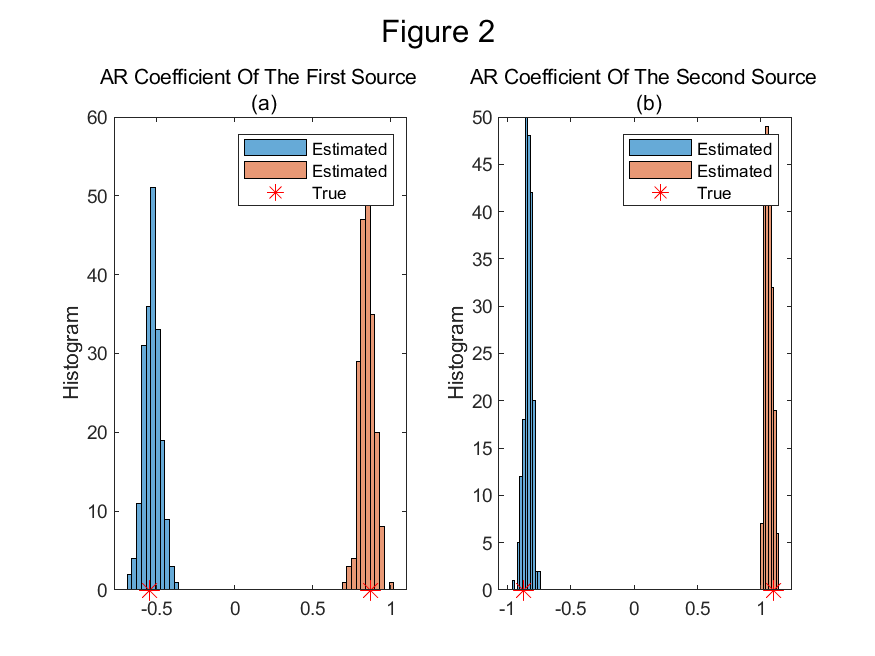
\includegraphics[width=0.75\textwidth]{Fig2.png}}
    \caption{Reproduced Figure 2, 2 sources, 3 sensors, $d_1 = \frac{\lambda}{4}$, SNR = 30 dB.}
    \label{fig:figure 1}
\end{figure}


\begin{figure}[htbp]
    \centerline{
    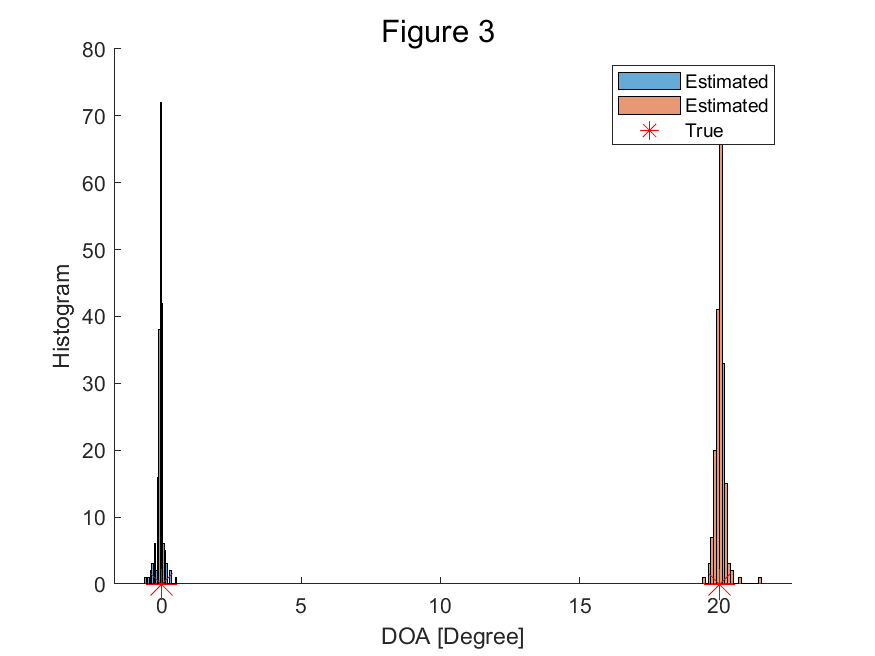
\includegraphics[width=0.75\textwidth]{Fig3.png}}
    \caption{Reproduced Figure 3, 2 sources, 3 sensors, $d_1 = \frac{\lambda}{4}$, SNR = 30 dB.}
    \label{fig:figure 2}
\end{figure}

\begin{figure}[htbp]
    \centerline{
    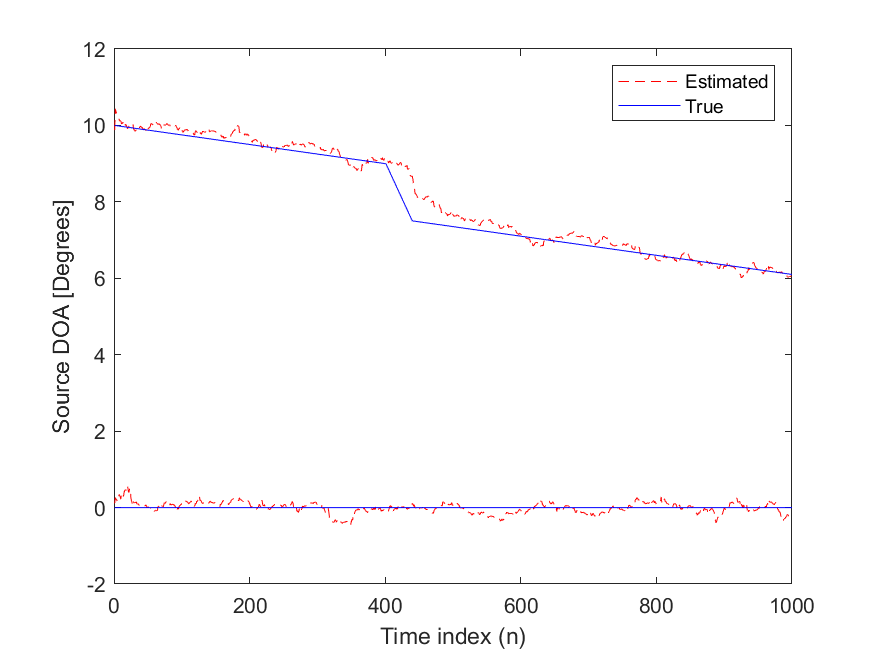
\includegraphics[width=0.75\textwidth]{Fig4.png}}
    \caption{Reproduced Figure 4, 2 sources, 5 sensors, $d_1 = \frac{\lambda}{2}$, $d_2 = \frac{\lambda}{2}$, $SNR = 10 dB$.}
    \label{fig:figure 3}
\end{figure}

\begin{figure}[htbp]
    \centerline{
    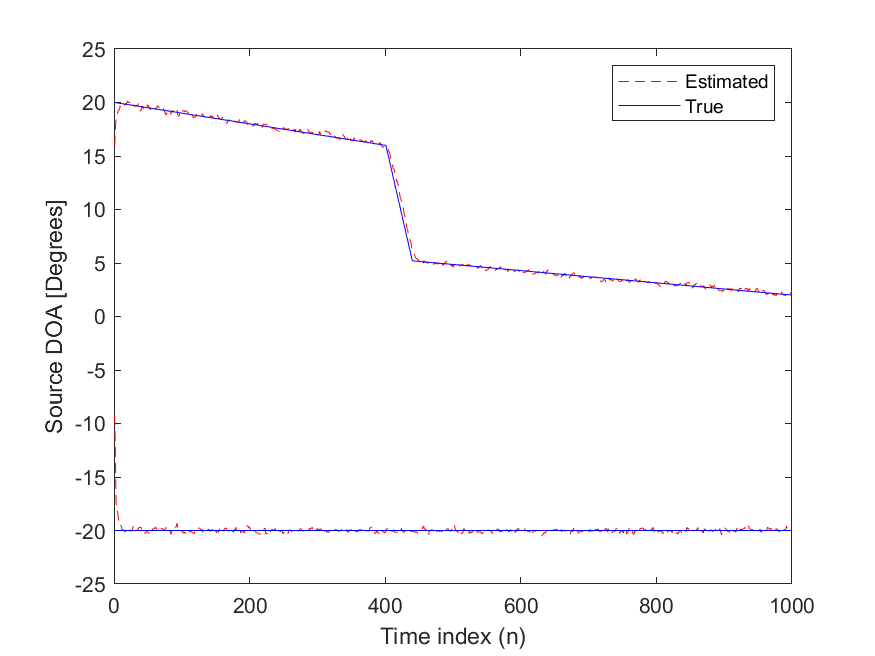
\includegraphics[width=0.75\textwidth]{Fig5.png}}
    \caption{Reproduced Figure 5, 2 sources, 5 sensors, $d_1 = \frac{\lambda}{2}$, $d_2 = \frac{\lambda}{2}$, $SNR = 30 dB$.}
    \label{fig:figure 4}
\end{figure}



\subsection{Parameter Experiments}
In this section, I experiment with different parameters to understand their effect on the algorithm's performance.
I examine the effect of SNR, the number of sources, the number of sensors, the order of the AR process.


\subsubsection{Effect of SNR}
I tested SNR values of 10,5,1 dB, The results are presented in Figure 5. \ref{fig:figure5}
It is interesting to see that the lower SNR mainly influences the DOA estimation and not AR parameter estimation.
Also, the effect of lower SNR is mainly bias in the estimated value with less noticeable effect on the variance of the estimation.



\begin{figure}[htbp]
    \centering
    \begin{subfigure}[AR Parameters]{
        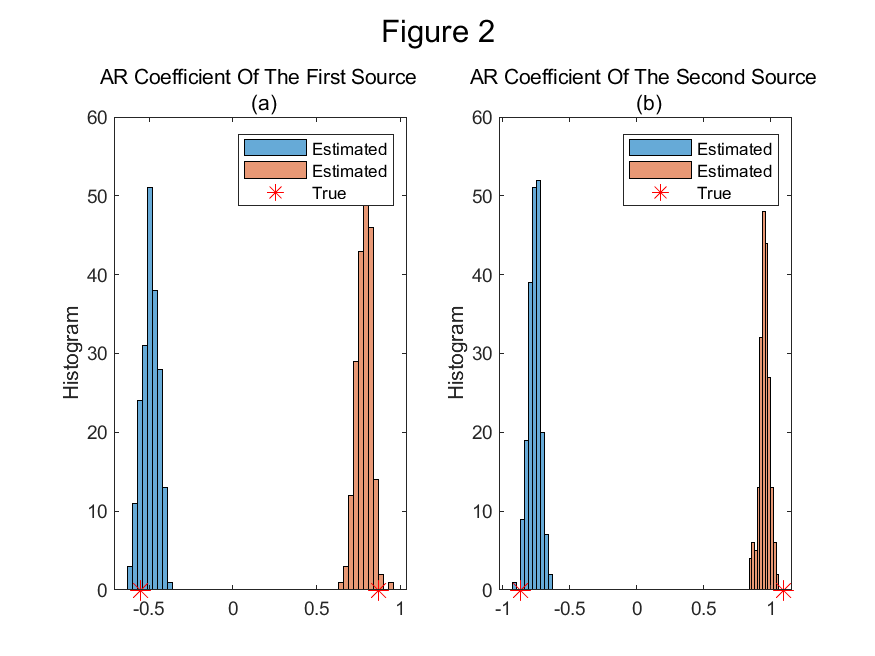
\includegraphics[width=0.3\textwidth]{Fig2_iSNR10.png}
        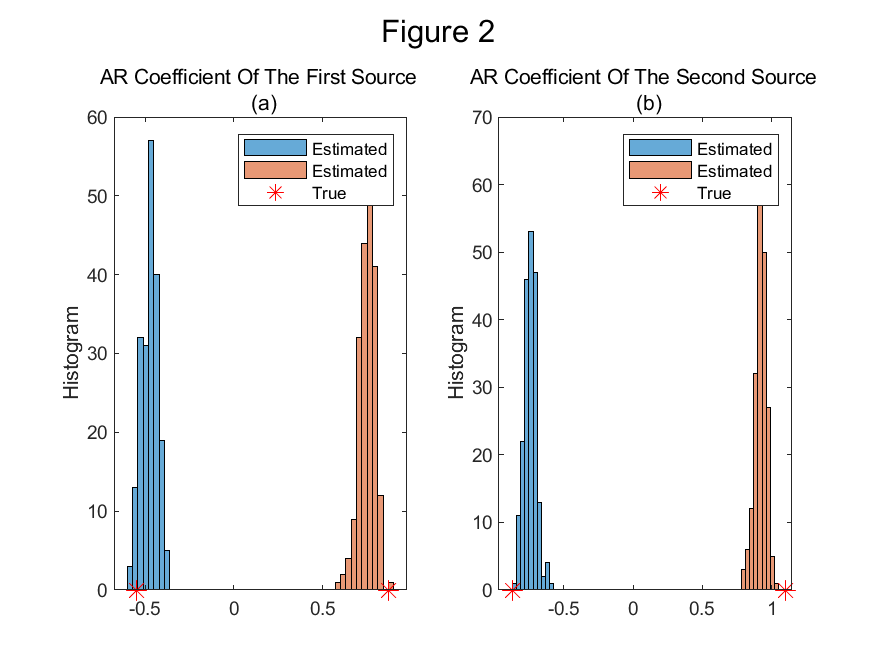
\includegraphics[width=0.3\textwidth]{Fig2_iSNR 5.png}
        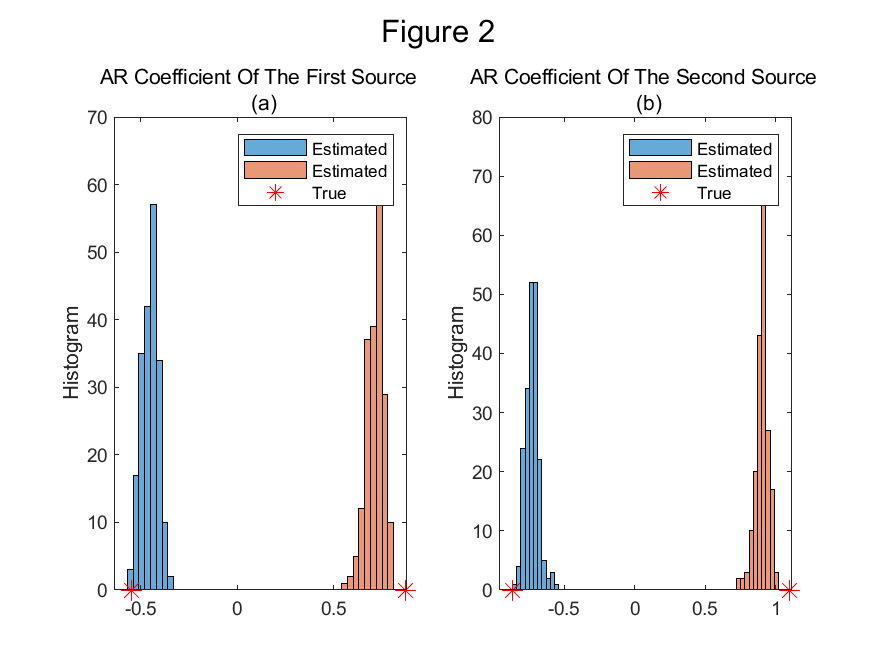
\includegraphics[width=0.3\textwidth]{Fig2_iSNR 1.png}}
    \end{subfigure}
    \medskip
    \begin{subfigure}[DOA Estimation]{
        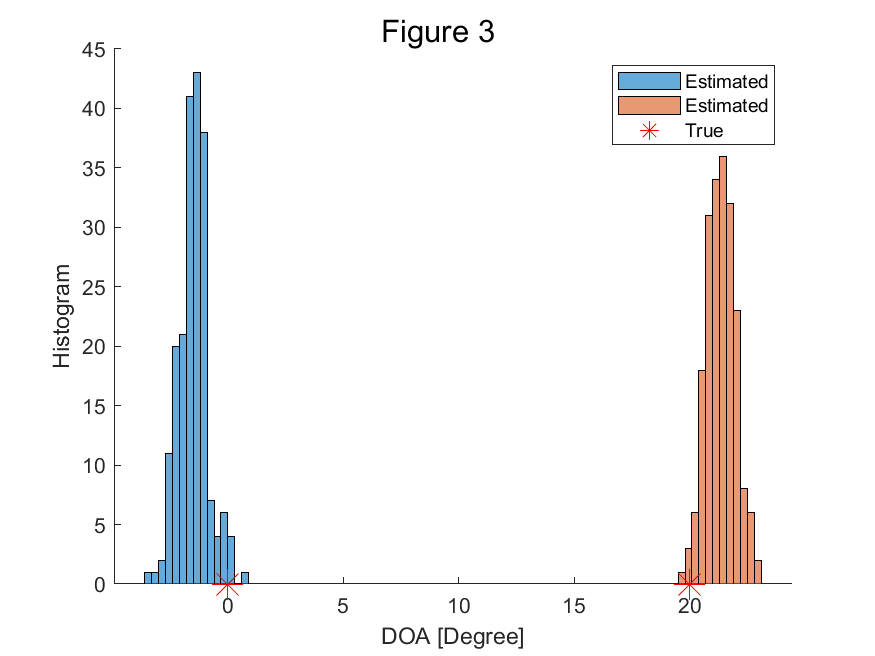
\includegraphics[width=0.3\textwidth]{Fig3_iSNR10.png}
        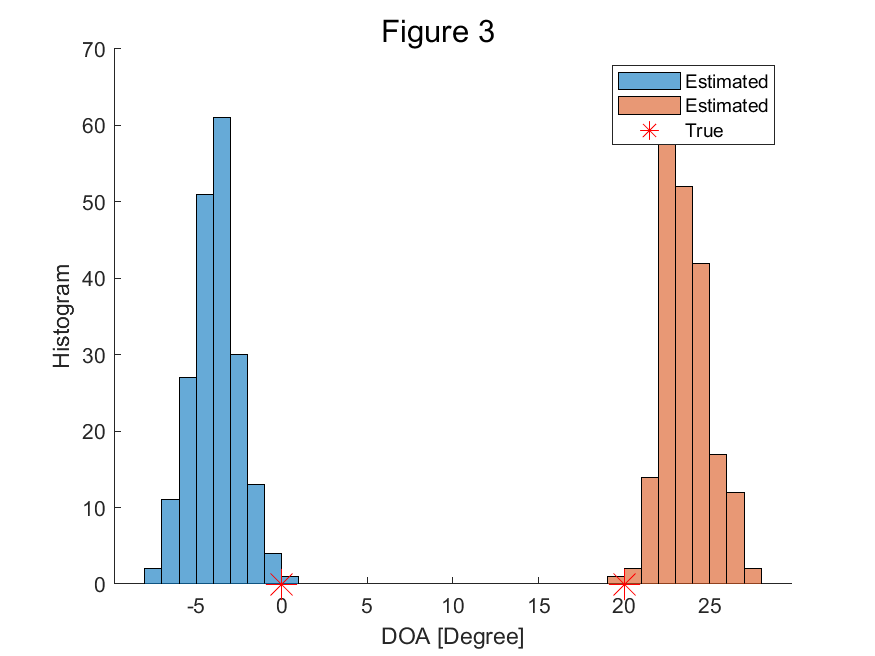
\includegraphics[width=0.3\textwidth]{Fig3_iSNR 5.png}
        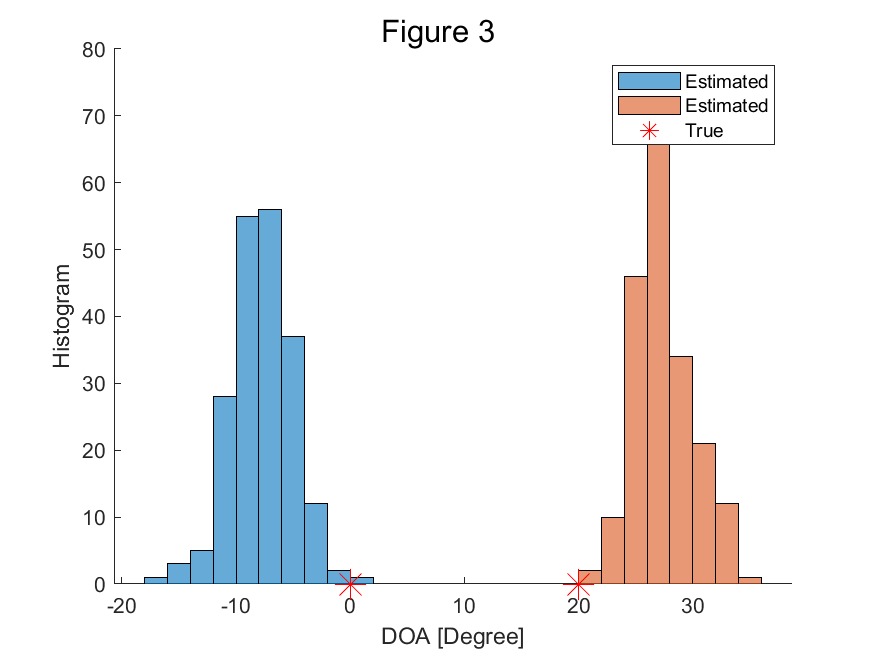
\includegraphics[width=0.3\textwidth]{Fig3_iSNR 1.png}}
    \end{subfigure}
    \caption[]{From left to right SNR = 10, 5, 1 dB.}
    \label{fig:figure5}
\end{figure}


\subsubsection{Effect of Number of Sensors}
I tested M (number of sensors) values of 2,3,4 The results are presented in Figure 6.
The effect of the number of sensors in mainly on the DOA estimation without much effect on the AR parameter estimation.'
DOA estimation with more sensors are less biased with significantly lower variance.
That is due to the averaging of the estimates of the pairs of rows in the regression model which reduces the estimation variance.
\ref{fig:figure6}
\begin{figure}[htbp]
    \centering
    \begin{subfigure}[AR Parameters]{
        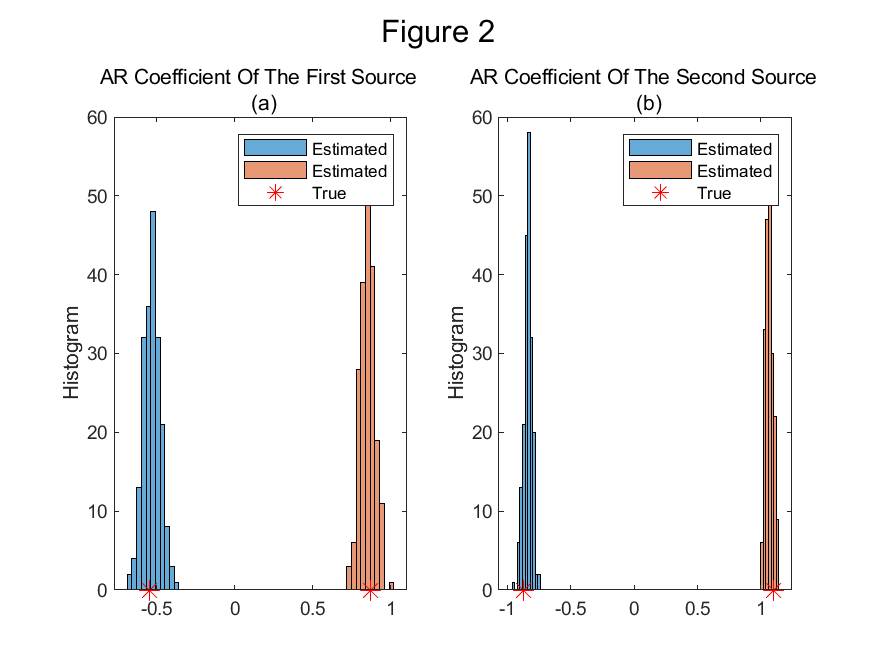
\includegraphics[width=0.3\textwidth]{Fig2_M 2.png}
        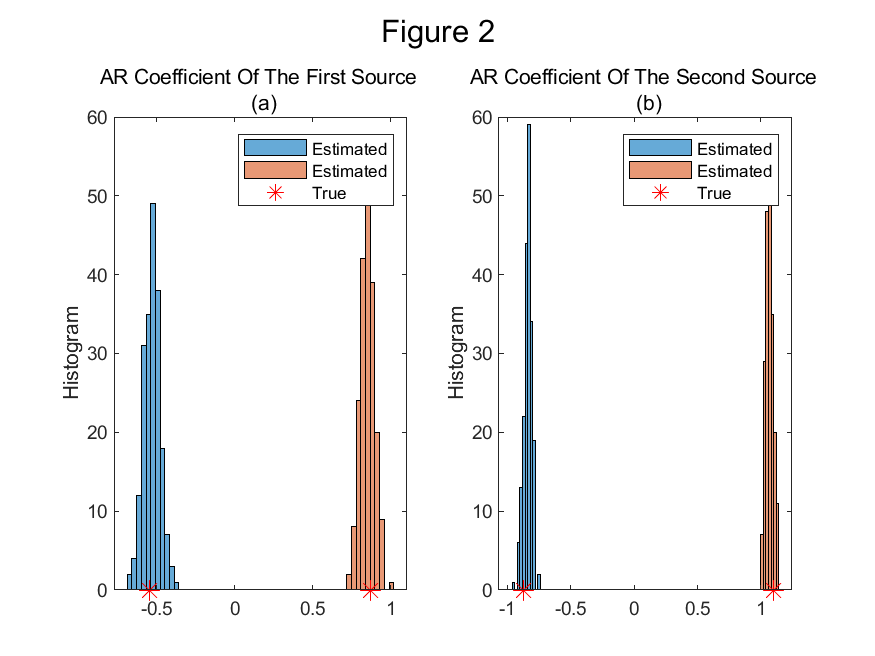
\includegraphics[width=0.3\textwidth]{Fig2_M 3.png}
        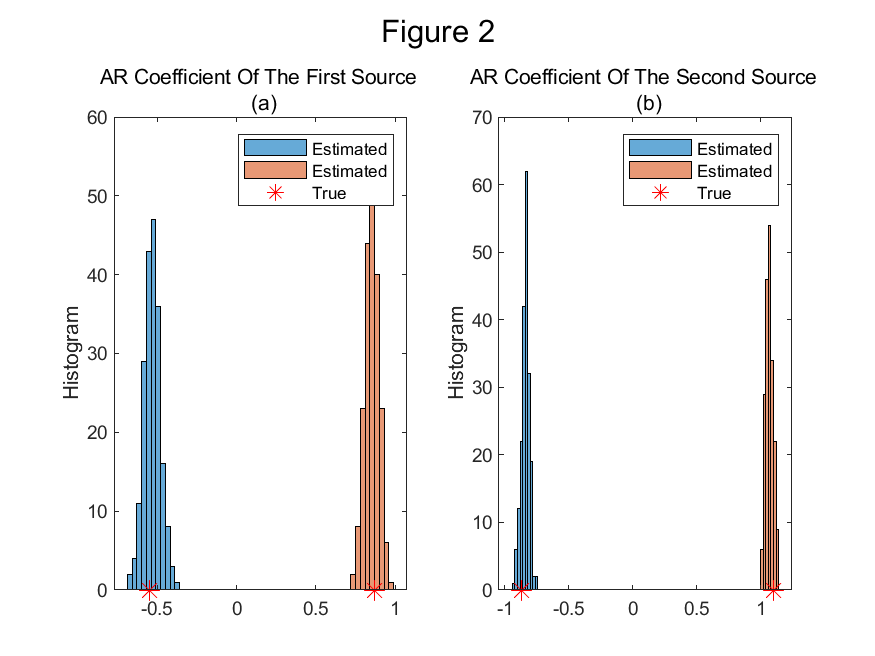
\includegraphics[width=0.3\textwidth]{Fig2_M 4.png}}
    \end{subfigure}
    \medskip
    \begin{subfigure}[DOA Estimation]{
        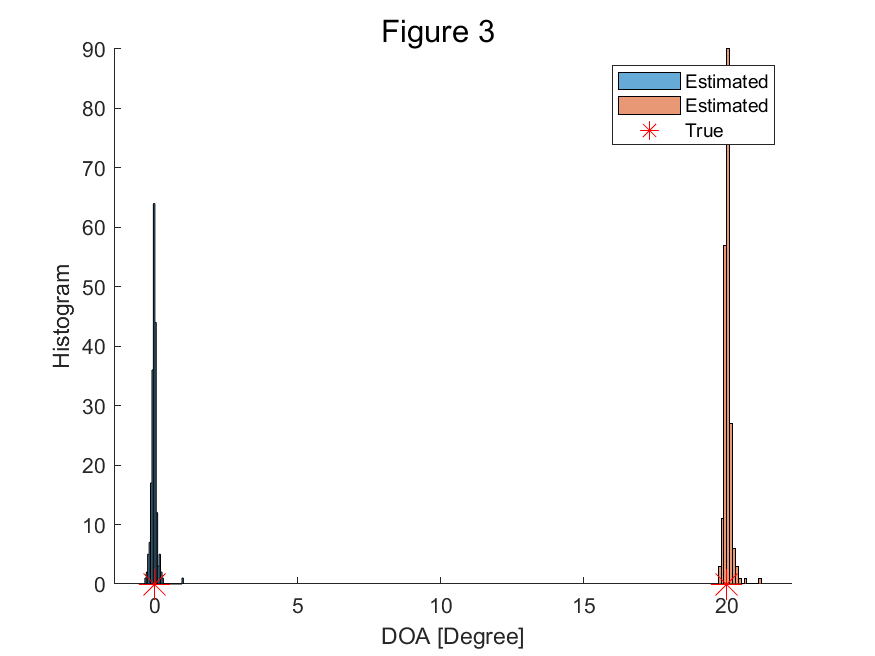
\includegraphics[width=0.3\textwidth]{Fig3_M 2.png}
        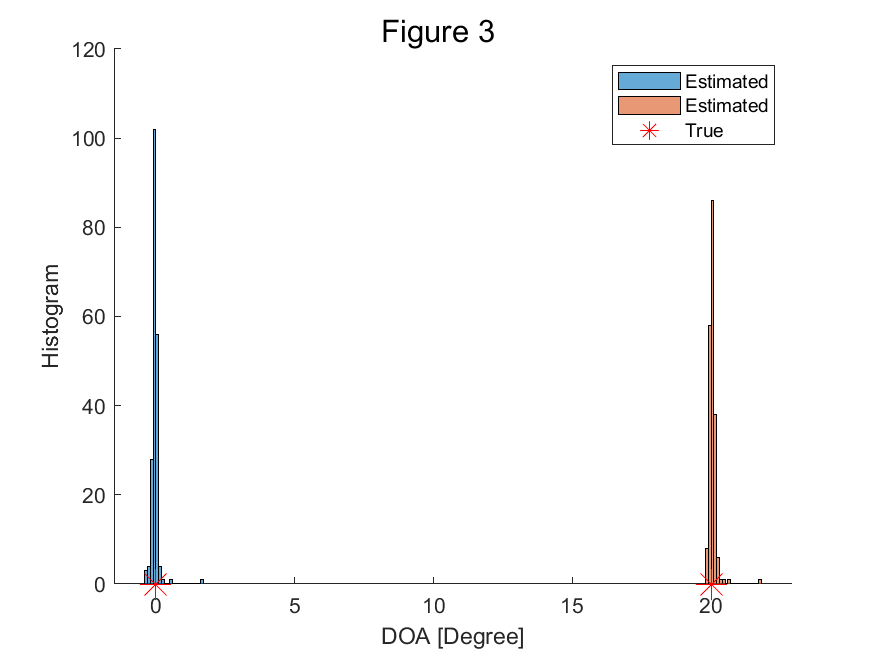
\includegraphics[width=0.3\textwidth]{Fig3_M 3.png}
        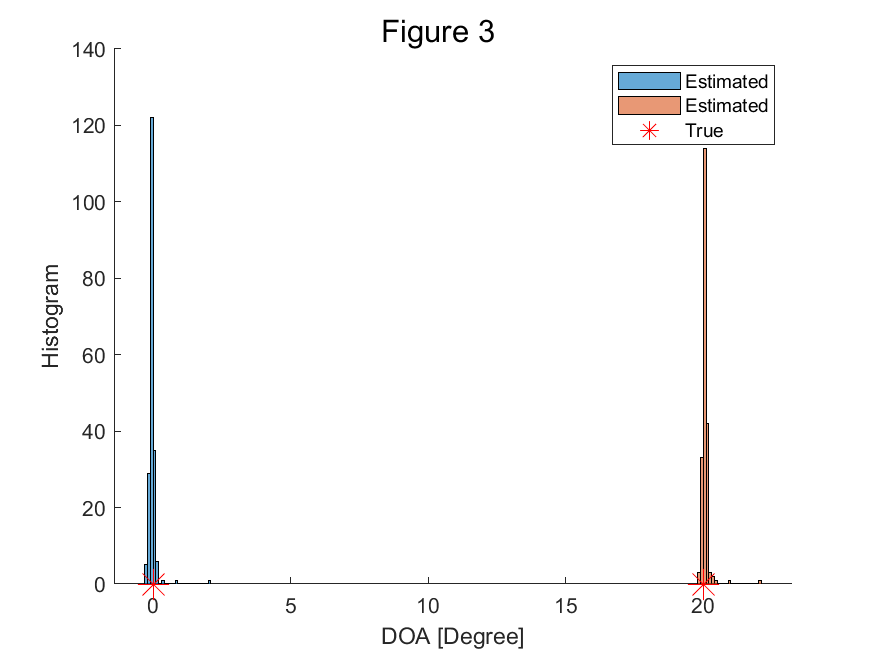
\includegraphics[width=0.3\textwidth]{Fig3_M 4.png}}
    \end{subfigure}
    \caption[]{From left to right M = 2, 3, 4}
    \label{fig:figure6}
\end{figure}

\subsubsection{Number of AR parameters}

I tested the effect of the number of AR parameters on the algorithm's performance.
I only tested with K = 3 for each source, the results are presented in Figure 7.
The algorithm is robust to the number of AR parameters with no significant effect on the performance.
\ref{fig:figure7}
\begin{figure}[htbp]
    \centering
    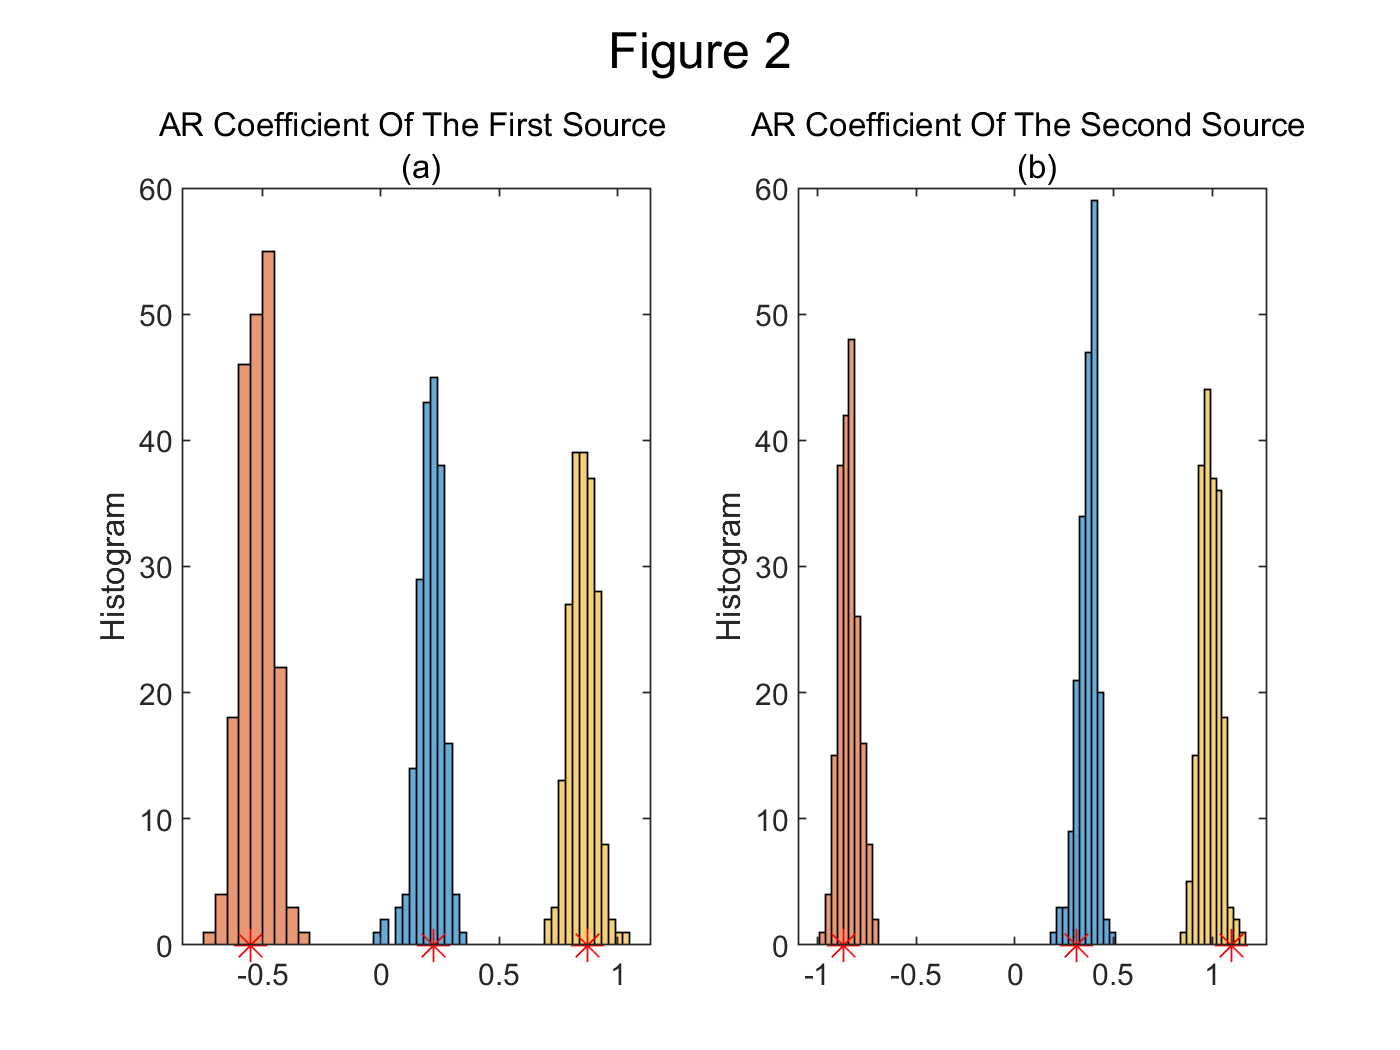
\includegraphics[width=0.3\textwidth]{Fig2_AR3.png}
    \caption[]{AR order = 3}
    \label{fig:figure7}
\end{figure}



\subsection[]{Speech Signal Performance}
I tested the algorithm on speech signals to demonstrate its performance on non-synthetic data.
First, I needed to estimate the order of the AR process for the speech signals, this is done using 
the partial auto-correlation function (PACF) of the speech signals.
By estimating the number of significant peaks outside the $95\%$ CI (Z-Score) in the PACF we can get a good estimate for the order of the process.
I estimated the order of the process to be 1 for the speech signals.
I then used the Yule-Walker method to get an initial estimate for the AR parameters.
The tests were done with N = 30 (window size), M = 2 sensors, K = 2 sources, SNR = 30,10,5 dB.
To simulate the desired SNR, assuming it is an AR process, I estimated the power of the signal and scaled it to be the desired SNR.
One source was moving from $40^\circ$ to $0^\circ$ and the other source was static at $-20^\circ$.
The results are presented in Figure 8 \ref*{fig:figure8}.

The results are quite impressive, the algorithm managed to estimate the DOA of the moving source quite accurately.
The algorithm also managed to estimate the DOA of the static source accurately.

\begin{figure}[htbp]
    \centering
    \begin{subfigure}{
        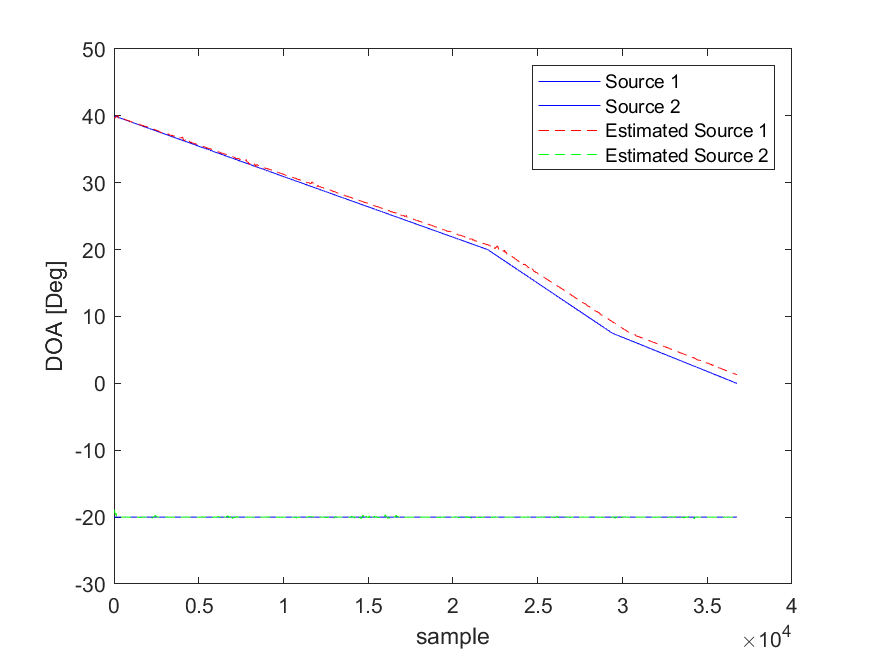
\includegraphics[width=0.3\textwidth]{DOA_Speech_iSNR30.png}
        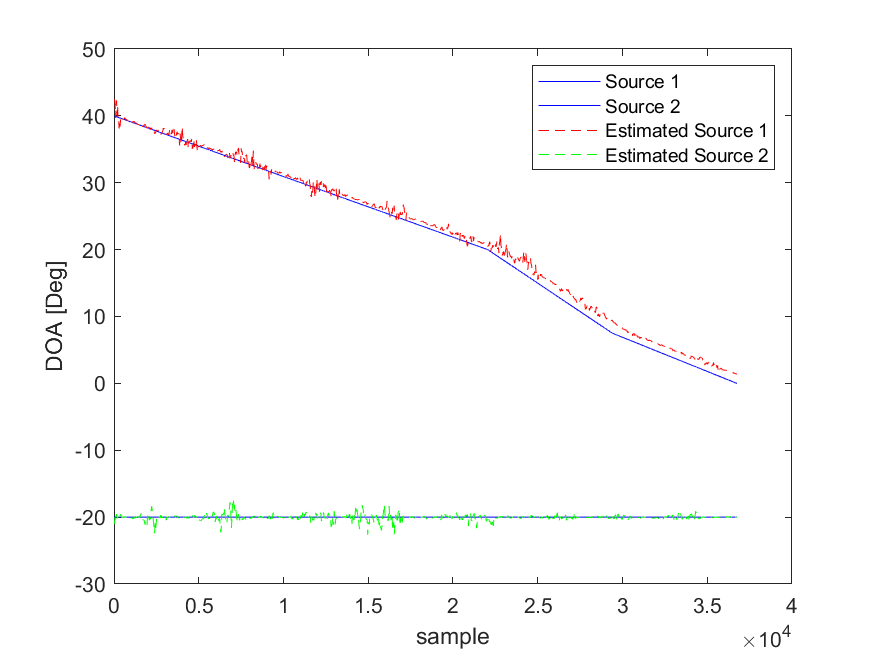
\includegraphics[width=0.3\textwidth]{DOA_Speech_iSNR10.png}
        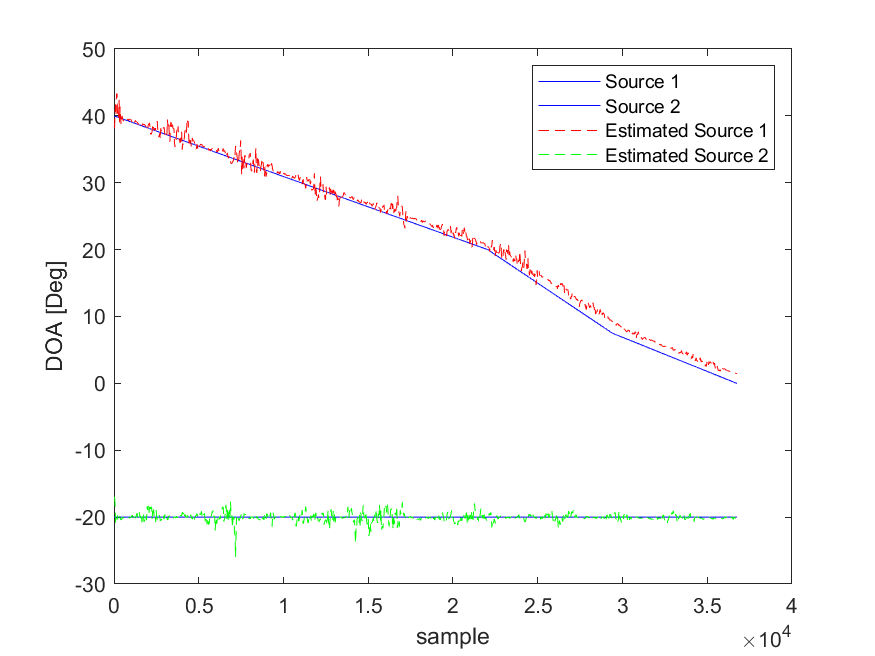
\includegraphics[width=0.3\textwidth]{DOA_Speech_iSNR 5.png}}
    \end{subfigure}
    \caption{Speech Signals Tracking Performance With SNR = 30, 10, 5 dB from left to right, AR order = 1.}  
    \label{fig:figure8}
\end{figure}

\begin{figure}[]
    \centering
    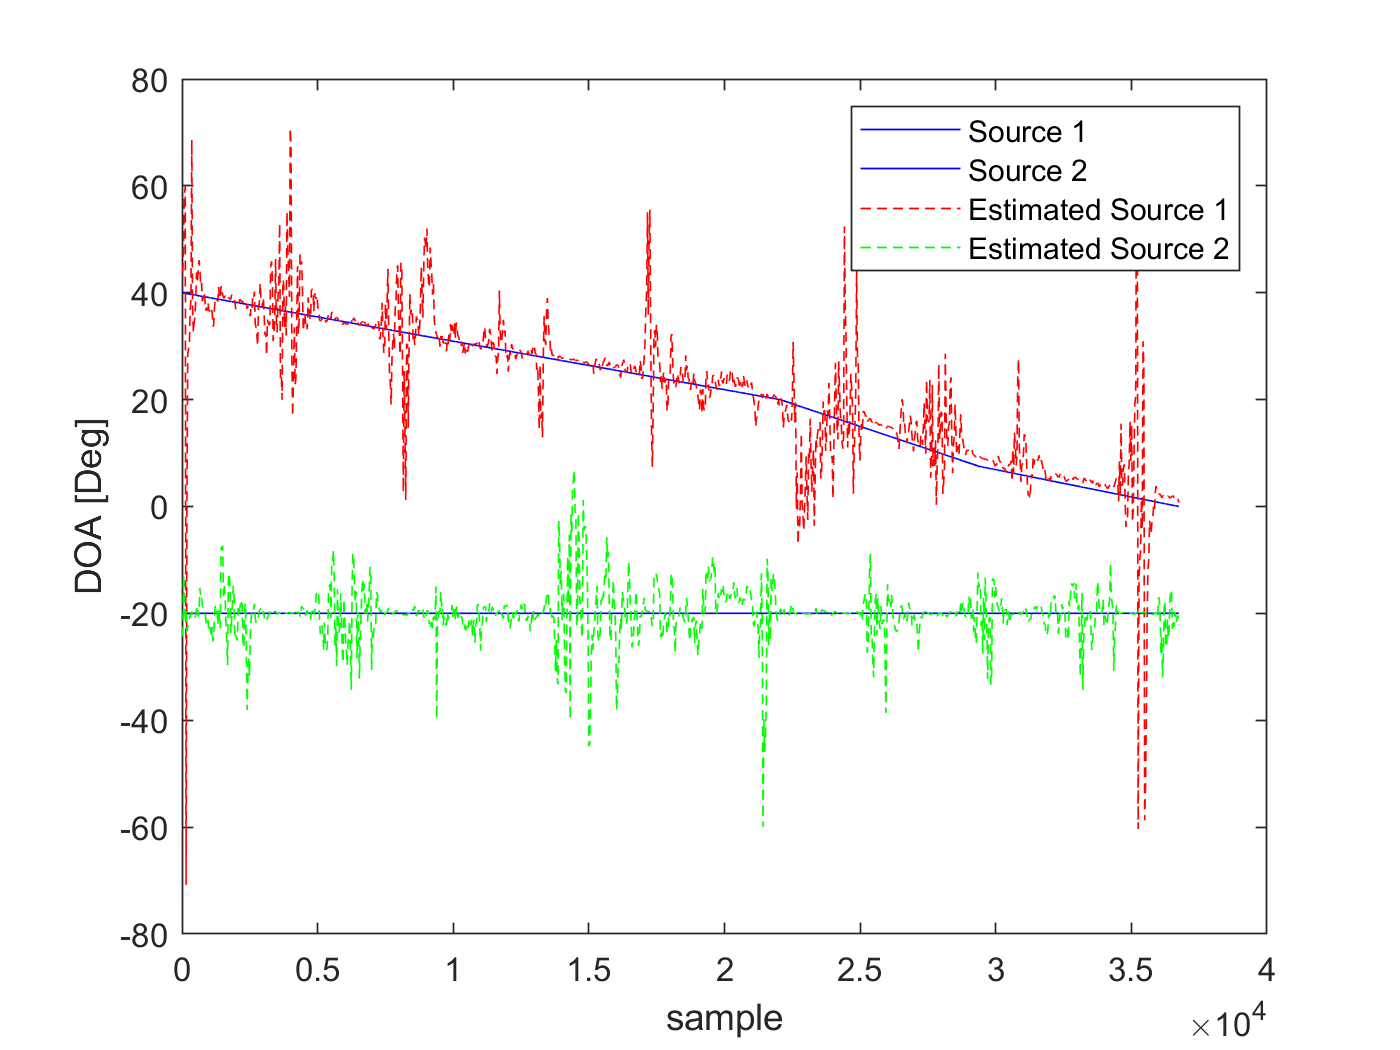
\includegraphics[width=0.7\textwidth]{DOA_Speech_iSNR30_Bad.png}
    \caption[]{AR order = 2, Algorithm performs poorly most of the time.}
    \label{fig:figure9}
\end{figure}

It is important to note that accurate estimation of the AR order is very crucial for the algorithm to work properly.
The algorithm completely fails when the order of the AR process is not known or estimated correctly as demonstrated in figure 9.
\ref*{fig:figure9}


\section{Summary}
Overall, the algorithm performed well on the simulated data and the speech signals. The algorithm is robust to parameter changes and can estimate the DOA of moving sources accurately.
There are several strengths of the algorithm:

\begin{enumerate}
    \item The is computationally efficient since it used recursive efficient algorithms, so it is suitable for real-time applications.
    \item Performs well even with only 2 sensors and multiple sources.
    \item Has high spatial resolution and can give accurate estimations for a wide range of angles and even when the sources are quite close.
    \item Works well even for small window sizes, so it can adapt more easily to changing dynamics.
\end{enumerate}    

There are several limitations to the algorithm:
\begin{enumerate}
    \item Assumes the sources are AR processes which may not be the case in practice.
    \item Fails when the order of the AR process is not known or estimated correctly.
    \item Relies on other algorithms/ heuristics to initiate the AR parameters.
\end{enumerate}

The algorithm has potential for real-world applications in speech enhancement, speaker localization, and tracking, and other applications that require DOA estimation and source separation.

% References
\bibliographystyle{plain}
\bibliography{references}
\end{document}


